
% Template for Elsevier CRC journal article
% version 1.0 dated 13 October 2009

% This file (c) 2009 Elsevier Ltd.  Modifications may be freely made,
% provided the edited file is saved under a different name

% This file contains modifications for Procedia Computer Science

%%%%%%%%%%%%%%%%%%%%%%%%%%%%%%%%%%%%%%%%%%%%%%%%%%%%%%%%%%%%%%%%%%%%%%%%%%

%% This template uses the elsarticle.cls document class and the extension package ecrc.sty
%% For full documentation on usage of elsarticle.cls, consult the documentation "elsdoc.pdf"
%% Further resources available at http://www.elsevier.com/latex

%%%%%%%%%%%%%%%%%%%%%%%%%%%%%%%%%%%%%%%%%%%%%%%%%%%%%%%%%%%%%%%%%%%%%%%%%%

%% The '1p' and 'times' class options of elsarticle are used for Elsevier CRC
\documentclass[1p,times]{elsarticle}

%% The `ecrc' package must be called to make the CRC functionality available
\usepackage{ecrc}

%% The ecrc package defines commands needed for running heads and logos.
%% For running heads, you can set the journal name, the volume, the starting page and the authors

%% set the volume if you know. Otherwise `00'
\volume{00}

%% set the starting page if not 1
\firstpage{1}

%% Give the name of the journal
\journalname{Procedia Computer Science}

%% Give the author list to appear in the running head
%% Example \runauth{C.V. Radhakrishnan et al.}
\runauth{M. Rivi et al.}

%% The choice of journal logo is determined by the \jid and \jnltitlelogo commands.
%% A user-supplied logo with the name <\jid>logo.pdf will be inserted if present.
%% e.g. if \jid{yspmi} the system will look for a file yspmilogo.pdf
%% Otherwise the content of \jnltitlelogo will be set between horizontal lines as a default logo

%% Give the abbreviation of the Journal.
\jid{procs}

%% Give a short journal name for the dummy logo (if needed)
\jnltitlelogo{Procedia Computer Science}

%% Hereafter the template follows `elsarticle'.
%% For more details see the existing template files elsarticle-template-harv.tex and elsarticle-template-num.tex.

%% Elsevier CRC generally uses a numbered reference style
%% For this, the conventions of elsarticle-template-num.tex should be followed (included below)
%% If using BibTeX, use the style file elsarticle-num.bst

%% End of ecrc-specific commands
%%%%%%%%%%%%%%%%%%%%%%%%%%%%%%%%%%%%%%%%%%%%%%%%%%%%%%%%%%%%%%%%%%%%%%%%%%

%% The amssymb package provides various useful mathematical symbols
\usepackage{amssymb}
%% The amsthm package provides extended theorem environments
%% \usepackage{amsthm}

%% The lineno packages adds line numbers. Start line numbering with
%% \begin{linenumbers}, end it with \end{linenumbers}. Or switch it on
%% for the whole article with \linenumbers after \end{frontmatter}.
%% \usepackage{lineno}

%% natbib.sty is loaded by default. However, natbib options can be
%% provided with \biboptions{...} command. Following options are
%% valid:

%%   round  -  round parentheses are used (default)
%%   square -  square brackets are used   [option]
%%   curly  -  curly braces are used      {option}
%%   angle  -  angle brackets are used    <option>
%%   semicolon  -  multiple citations separated by semi-colon
%%   colon  - same as semicolon, an earlier confusion
%%   comma  -  separated by comma
%%   numbers-  selects numerical citations
%%   super  -  numerical citations as superscripts
%%   sort   -  sorts multiple citations according to order in ref. list
%%   sort&compress   -  like sort, but also compresses numerical citations
%%   compress - compresses without sorting
%%
%% \biboptions{comma,round}

% \biboptions{}

% if you have landscape tables
%%%\usepackage[figuresright]{rotating}

% put your own definitions here:
%   \newcommand{\cZ}{\cal{Z}}
%   \newtheorem{def}{Definition}[section]
%   ...

% add words to TeX's hyphenation exception list
%\hyphenation{author another created financial paper re-commend-ed Post-Script}

% declarations for front matter

\newcommand{\aj}{AJ}
\newcommand{\apj}{ApJ}
\newcommand{\apjl}{ApJ}
\newcommand{\apjs}{ApJS}
\newcommand{\aap}{A\&A}
\newcommand{\aaps}{A\&AS}
\newcommand{\mnras}{MNRAS}
\newcommand{\nat}{Nature}
\newcommand{\araa}{ARAA}
\newcommand{\prd}{Phys. Rev. D}
\newcommand{\pasj}{PASJ}
\newcommand{\pasp}{PASP}
\newcommand{\physrep}{Phys. Rep.}


\begin{document}

\begin{frontmatter}

%% Title, authors and addresses

%% use the tnoteref command within \title for footnotes;
%% use the tnotetext command for the associated footnote;
%% use the fnref command within \author or \address for footnotes;
%% use the fntext command for the associated footnote;
%% use the corref command within \author for corresponding author footnotes;
%% use the cortext command for the associated footnote;
%% use the ead command for the email address,
%% and the form \ead[url] for the home page:
%%
%% \title{Title\tnoteref{label1}}
%% \tnotetext[label1]{}
%% \author{Name\corref{cor1}\fnref{label2}}
%% \ead{email address}
%% \ead[url]{home page}
%% \fntext[label2]{}
%% \cortext[cor1]{}
%% \address{Address\fnref{label3}}
%% \fntext[label3]{}

\dochead{}
%% Use \dochead if there is an article header, e.g. \dochead{Short communication}



\title{High Performance Visualization of astrophyisical data using Splotch}

%% use optional labels to link authors explicitly to addresses:
%% \author[label1,label2]{<author name>}
%% \address[label1]{<address>}
%% \address[label2]{<address>}

\author{Marzia Rivi}
\ead{m.rivi@cineca.it}
\address{CINECA, Via Magnanelli 6/3, Casalecchio di Reno, Italy}

\author{Zhefan Jin}
\ead{Zhefan.Jin@port.ac.uk}
\address{School of Creative Technologies, University of Portsmouth, Portsmouth, United Kindom}

\author{Klaus Dolag}
\ead{kdolag@MPA-Garching.MPG.DE}
\address{Max-Planck-Institut f\"ur Astrophysik, Karl-Schwarzschild Strasse 1, Garching bei M\"unchen, Germany}

\author{Claudio Gheller }
\ead{c.gheller@cineca.it}
\address{CINECA, Via Magnanelli 6/3, Casalecchio di Reno, Italy}

\author{Mel Krokos }
\ead{mel.krokos@port.ac.uk}
\address{...}

\author{Martin Reinecke}
\ead{martin@MPA-Garching.MPG.DE}
\address{Max-Planck-Institut f\"ur Astrophysik, Karl-Schwarzschild Strasse 1, Garching bei M\"unchen, Germany}

\begin{abstract}

Current technological advances impact profoundly on the unprecedented
growth in the quality and quantity of astrophysical datasets. The main
characteristic is extremely large sizes (many GBs) while forthcoming
next-generation astrophysical datasets are expected to exhibit
massively large sizes (many TBs). Visual data exploration and
discovery tools are robust instruments to rapidly and intuitively
inspecting very large-scale datasets to identify regions of interest
within which to apply time-consuming algorithms.  This paper reports
on recent developments for a high performance implementation of
Splotch, our previously developed ray-tracing algorithm for effective
visualization of large-scale astrophysical datasets coming from
particle-based simulations.  We discuss several approaches for
paralellizing Splotch to suit multicore CPUs and CUDA-enabled GPUs. We
present benchmarks of our implementations, specifically discussing the
MilleniumII simulation. Finally we summarise the work concluding with
pointers to future developments.

\end{abstract}

\begin{keyword}
%% keywords here, in the form: keyword \sep keyword


Visual Discovery \sep Splotch \sep Large-Scale Particle-Based
Numerical Simulations\sep High-Performance Visualization \sep
OpenMP \sep CUDA-enabled GPUs\sep MilleniumII Simulation 


%% PACS codes here, in the form: \PACS code \sep code

%% MSC codes here, in the form: \MSC code \sep code
%% or \MSC[2008] code \sep code (2000 is the default)

\end{keyword}

\end{frontmatter}

%%
%% Start line numbering here if you want
%%
% \linenumbers

\section{Introduction}
\label{intro}

Nowadays the technological advances in instrumentation and computing
capability impact profoundly on the dramatic growth in the quality and
quantity of astrophysical datasets obtained from observational
instruments, e.g.  sky surveys \cite{sdss}, \cite{lofar}, or
large-scale numerical simulations, e.g. the MillenniumII
simulation \cite{2009MNRAS.398.1150B}.

The main characteristic of
modern astrophysical datasets is extremely large sizes (in the order
of hundreds of GBs) requiring storage in extremely large-scale
distributed databases. The forthcoming next-generation astrophysical
datasets are expected to exhibit massively large sizes (in the order
of hundreds of TBs), e.g. \cite{lsst}.

To obtain a comprehensive insight into modern astrophysical datasets
astronomers employ sophisticated data mining algorithms often at high
computational costs. Visual data exploration and discovery tools are
then exploited in order to rapidly and intuitively inspect very
large-scale datasets to identify regions of interest within which to
apply time-consuming algorithms.  Such tools are based on a
combination of meaningful data {\it visualizations} and user
interaction with them.  

For example, meaningful visualizations can be generated through
display of multiple properties simultaneously together with customized
look up tables for colouring. This can be a very intuitive and
effective way of discovering and understanding rapidly brand new
correlations, similarities and data patterns. For on-going processes,
e.g. a numerical simulation in progress, advanced visual data
exploration and discovery allow constant monitoring and - if anomalies
are discovered - correcting the simulation parameters  thus saving
valuable time and resources. For such reasons the astronomical
community always dedicated special attention to graphical and
visualization tools either driving their evolution or even being
directly involved in developing them.

The data exploration tools traditionally employed by astronomers are
limited either on processing and displaying of 2D images
(e.g. IRAF \cite{iraf}, by NOAO; ESO-MIDAS \cite{midas} by the
European Southern Observatory; SaoImage \cite{sao} by the Smithsonian
Astrophysical Observatory and GAIA \cite{gaia} by ESO) or on
generation of meaningful 2D and 3D plots (e.g. Gnuplot \cite{gnuplot};
SuperMongo \cite{supermongo} and IDL \cite{idl} by ITT Visual
Information). There is a plethora of other tools, for details the
reader is referred to dedicated literature surveys,
e.g. \cite{survey}.

To overcome the shortcomings of traditional tools, a new generation of
software packages is now emerging providing astronomers with robust
instruments in the context of large-scale astrophysical datasets,
e.g. \cite{paraview}, \cite{aladin}, \cite{topcat}, \cite{visivo1}, \cite{3dslicer}, \cite{splash}
and \cite{visit}. The underlying principles are exploitation of high
performance architectures (i.e. multicore CPUs and powerful graphics
boards), interoperability (i.e. allowing different applications, each
specialized for different purposes, to operate on shared datasets) and
collaborative workflows (i.e. permitting several users to work
simultaneously for exchanging information and visualization
experiences).

ParaView \cite{paraview} was developed specifically for handling
large-scale datasets efficiently by exploiting distributed
memories. Aladin \cite{aladin} is an interactive sky atlas for
visualization of astronomical images supporting access to astronomical
databases (such as Simbad \cite{simbad} and
VizieR \cite{vizier}). TopCat \cite{topcat} is an application that
includes several tools for analysis and visualization of astronomical
tables. VisIVO \cite{visivo1} is an integrated suite of tools and
services specifically designed for multidimensional
visualisation. VisIVO Server is a recent development for visualization
of large-scale astrophysical datasets \cite{visivo2}.

Other examples of new-generation software packages for astrophysical
visualization are 3D slicer \cite{3dslicer} capable of displaying
volumetric datasets and user defined cut throughs,
SPLASH \cite{splash} specifically designed in the context of
astrophysical simulations and VisIt \cite{visit} which is a parallel
visualization and data analysis application supporting a rich set of
visualisation features, e.g. displaying of scalar and vector fields
defined on 2D or 3D structured and unstructured meshes. 

This paper describes a high performance implementation of
Splotch \cite{2008NJPh...10l5006D}, our previously developed
ray-tracing algorithm for effective visualization of large-scale
astrophysical datasets coming from particle-based computer
simulations. N-Body simulations constitute prime examples of
particle-based simulations, typically associated with very large-scale
datasets, e.g. the MillenniumII
simulation \cite{2009MNRAS.398.1150B}. This is a simulation of the
evolution of a meaningful fraction of the universe by means of 10
billion fluid elements (or particles) interacting with each other
through gravitational forces. The typical size of a snapshot of the
MillenniumII simulation is about 400 GBs representing a particle's ID,
position, velocity together with additional properties, e.g. local
smoothing length, density and velocity dispersion. For further details
on the MillenniumII simulation the reader is referred
to \cite{2009MNRAS.398.1150B}.

The fundamentals and the traditional sequential operation of
Splotch \cite{2008NJPh...10l5006D} are reviewed in section 2. Section
3 discusses our strategy for paralellizing Splotch based on different
approaches that are suitable for a variety of underlying architecture
configurations. Our implementations are Single Instruction Multiple
Data (SIMD) designs founded on the MPI library \cite{mpi} in order to
support distributed multicore CPUs, the OpenMP \cite{openmp} for
supporting shared memory nodes and finally CUDA \cite{cuda} for
exploiting not only currently available but also forthcoming
next-generation multiple GPUs. The advantage of adopting several
parallelization solutions is that we can deploy them simultaneously on
hybrid architectures, e.g. mixed hardware architectures consisting of
a large number of multicore CPUs and CUDA-enabled GPUs. Benchmarks for
our paralellization designs and a discussion on the MilleniumII
visualization are presented in section 4. Finally section 5 outlines a
summary of our work and includes pointers to future developments. 


\section{The Splotch Algorithm}
\label{splotch}

\begin{figure}
\begin{center}
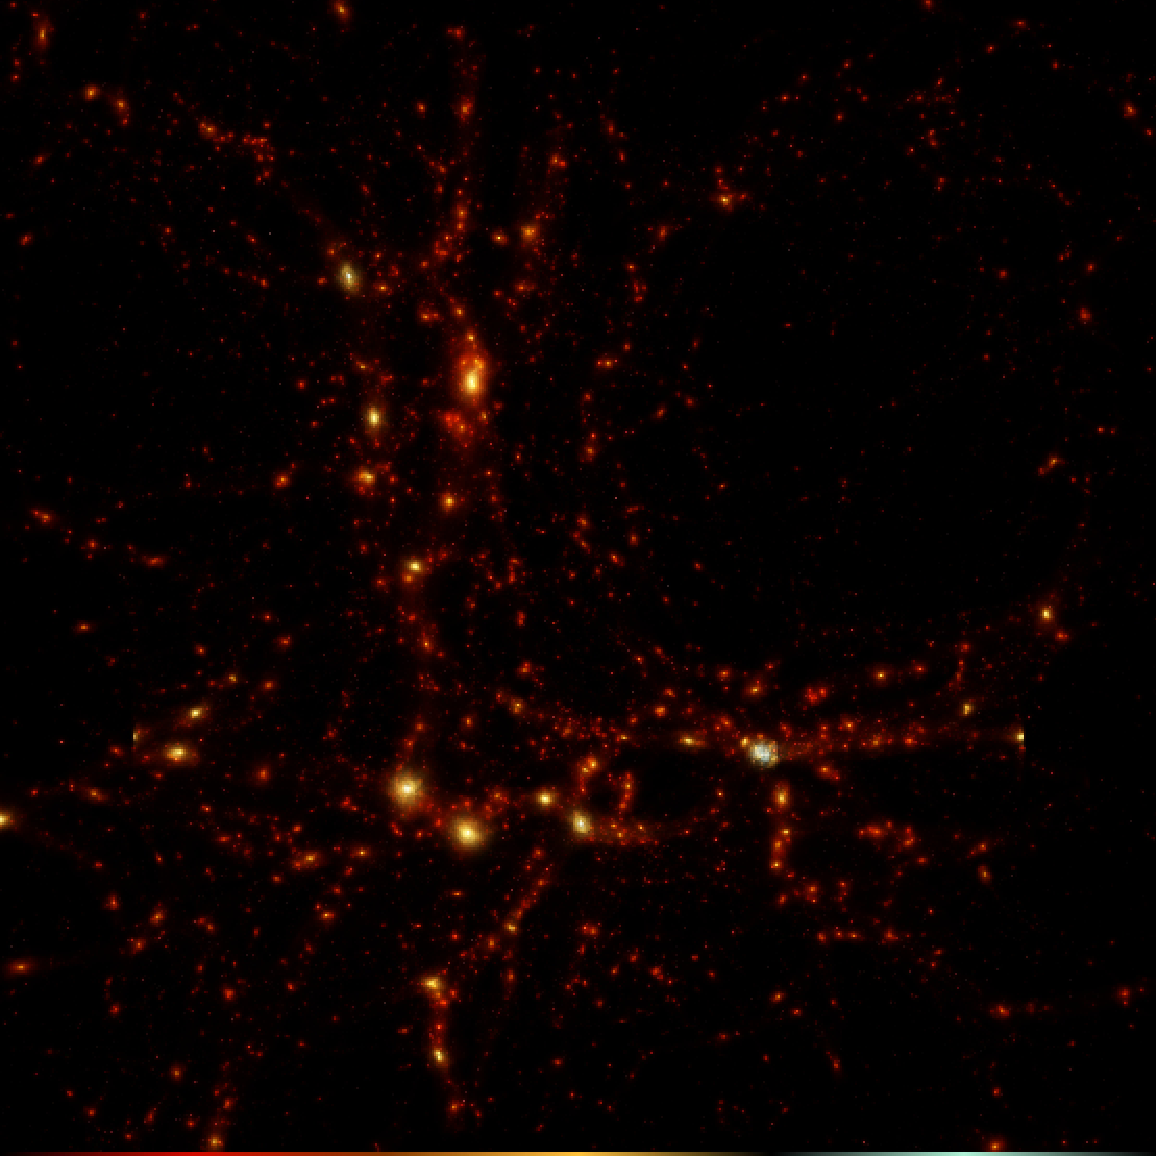
\includegraphics[width=0.49\textwidth]{millenium2_veldisp.pdf}
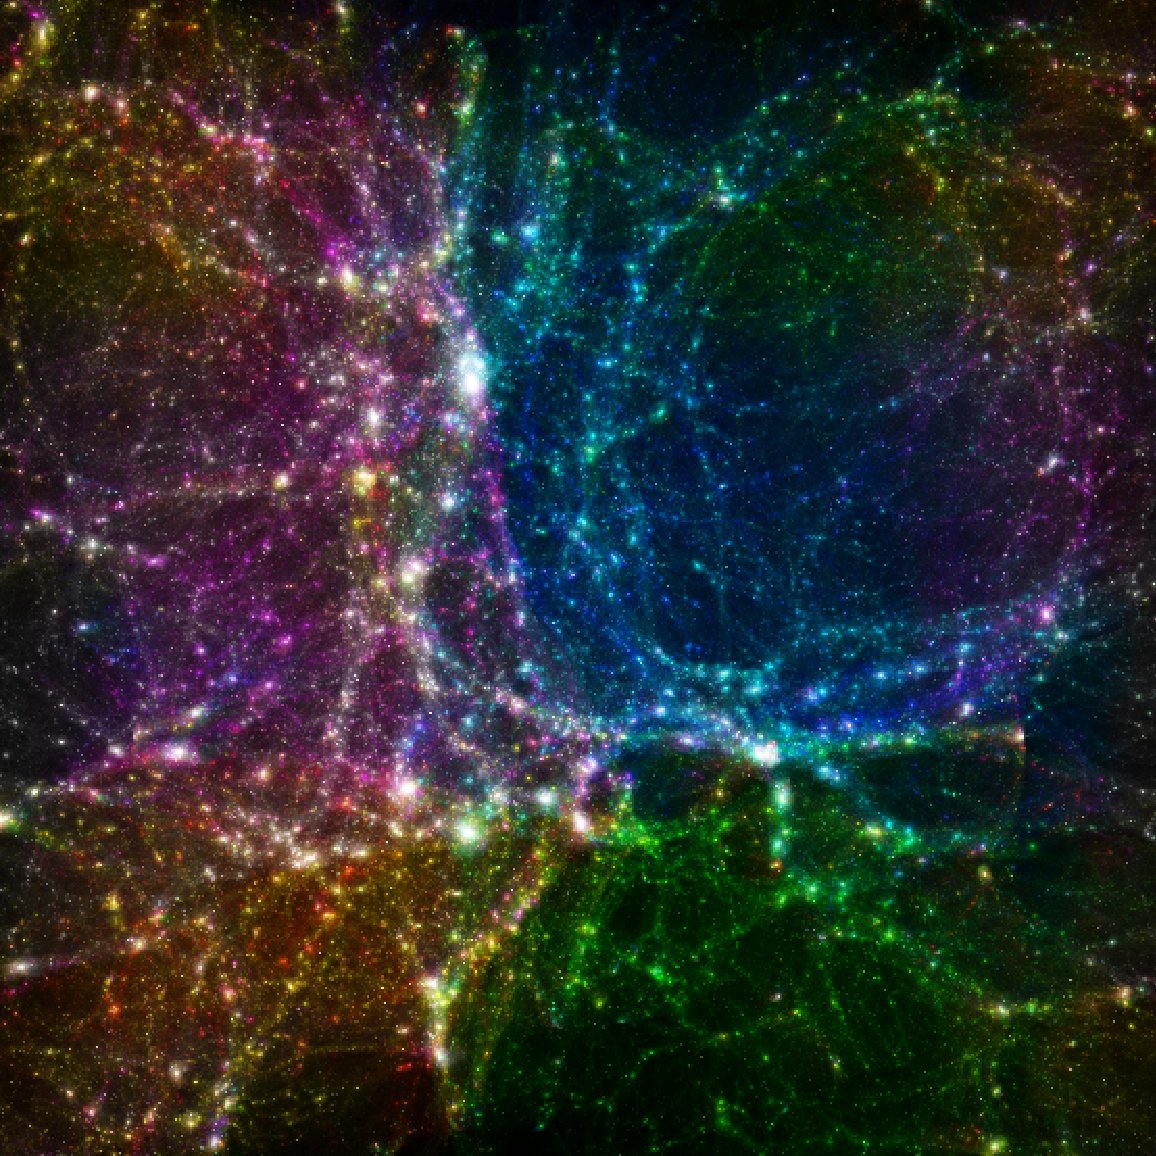
\includegraphics[width=0.49\textwidth]{millenium2_vel.pdf}
\end{center}
\caption{Shown are vizualisation of the MilleniumII simulation \cite{2009MNRAS.398.1150B} using
the velocity dispersion (left panel) and the three dimensional velocity (right panel) of the
particles for the color transfere function. The inlay shows a zoom on one the most rich structure
inside the simulation.}\label{mil2}
\end{figure}

The rendering algorithm of {\tt Splotch} is generally designed to handle
point-like particle distributions. Such tracer particles can be smoothed
to obtain a contineous field, most commonly the $B_2$-Spline \cite{1985A&A...149..135M}
\begin{equation}
   W(x,h)=\frac{8}{\pi h^3}\left\{\begin{array}{ll}
      1 - 6 \left(\frac{x}{h}\right)^2 + 6 \left(\frac{x}{h}\right)^3 \;\;& 0 \le \frac{x}{h} < 0.5 \\
      2 \left(1 - \frac{x}{h}\right)^3                              & 0.5 \le \frac{x}{h} < 1 \\
      0                                                             & 1 \le \frac{x}{h} \\
   \end{array} \right. , \label{SPH:kern}
\end{equation}
where $h$ is the local smoothing length, which is typically defined in a way
that every particle overlaps with $\approx 32$ neighbors. Therefore, the rendering is
based on the following assumptions:

\begin{itemize}
\item The contribution to the matter density by every particle can
be described as a Gaussian distribution of the form 
$\rho_p(\vec r)=\rho_{0,p}\exp(-r^2/\sigma_p^2)$.\footnote{Note that the
$b_2$-Spline kernel used in SPH has a shape very similar to the Gaussian distribution.} In
practice, it is much more handy to have a compact support of the
distribution, and therefore the distribution is set to zero at a given
distance of $f\cdot\sigma_p$. Following the approach often used to vizualice 
cosmological simulation we choose $f$ in such a way that
$f\cdot\sigma_p$ is related to the smoothing length $h$, i.e.
to fulfill $h \approx f\cdot\sigma_p$. Therefore rays passing
the particle at a distance larger than $f\cdot\sigma_p$ will be practically
unaffected by the particle's density distribution.
\item We use three ``frequencies'' to describe the red, green and blue
components of the radiation, respectively. These are treated independently.
\item The radiation intensity $\bf{I}$\footnote{Here we treat all
intensities as vectors with r,g and b components.} along a ray through the simulation
volume is modeled by the well known radiative transfer equation
\begin{equation}
\frac{d\bf{I}(x)}{dx}=(\bf{E}_p-\bf{A}_p\bf{I}(x))\rho_p(x),
\end{equation}
which can be found in standard textbooks \cite{1991par..book.....S}.
Here, $\bf{E}_p$ and $\bf{A}_p$ describe the strength of radiation emission and absorption
for a given particle for the three rgb-colour components. In general it is recommended to
set $\bf{E}_p=\bf{A}_p$, which typically produces visually appealing images; for special
effects, however, independent emission and absorption coefficients can be used. Specially typically
a small gray component (e.g. a small, constant addition to the rgb-components) can be added 
to the absortpion of each particle ($\bf{A}_p$) to improve the three dimensional impression.
In general the coefficients can vary between particles, and are typically chosen as a function 
of a characteristic particle property. If a scalar quantity is choosen (e.g. the particle temperature, 
density, velocity dispersion, etc.), the mapping to the three components of $\bf{E}$ and $\bf{A}$ (for red, green and blue)
is typically achieved via a transfere function, realized by a colour look-up table or palette, which can
be provided to the ray-tracer as an external file to allow a maximum of flexibility. If a
vector quantity is chosen (r.g. velocity, magnetic field, etc.), the three components of the vectors
can be maped to the three components of $\bf{E}$ and $\bf{A}$ (for red, green and blue). Additional 
to the color, the intensity of each particle can be aditional modulated proportional to another
scalar property (e.g. density, etc.).
\end{itemize}

Assuming that absorption and emission are homogeneously mixed it
can be shown that, whenever a ray traverses a particle, its intensity
change is given by
\begin{equation}
\label{i_change}
\bf{I}_{\mbox{after}}=(\bf{I}_{\mbox{before}}-\bf{E}_p/\bf{A}_p)
\exp(-\bf{A}_p\int_{-\infty}^\infty\rho_p(x)dx) + \bf{E}_p/\bf{A}_p
\end{equation}
The integral in this equation is given by
$\rho_{0,p}\sigma_p\exp{(-d_0^2/\sigma_p^2)}\sqrt{\pi}$, where $d_0$
is the minimum distance between the ray and the particle center.

Under the assumption that the particles do not overlap, the intensity
reaching the observer could simply be calculated by applying this formula to
all particles intersecting with the ray, in the order of decreasing distance
to the observer. In reality, of course, the particles do overlap, but since
the relative intensity changes due to a single particle can be assumed to be
very small, this approach can nevertheless be used in good approximation.

Figure \ref{mil2} shows a vizualisation example of a large simulation 
containing 10 billion particles.

\section{Parallel Implementation}
\label{parallel}

The Splotch code workflow consists in a number of steps,
% which can be 
summarized as follows:
\begin{enumerate}
\item Read data from one or more files;
\item process data for rescaling, normalization etc.;
\item render data;
\item save the final image.
\end{enumerate}
All these steps can be parallelized according to the same strategy, based on a SIMD approach. 
This consists in 
distributing the data in a balanced way between the different computing elements.
Each computing element performs the same operations on its subset of data contributing 
to the final (unique) image. 

The parallel implementation has been accomplished using different approaches, suitable 
for different hardware architectures and software environments. The MPI library \cite{mpi} 
has been used to define the overall data and work distribution characterization. Data are
read in chuncks of the same (or similar) size from each processor in the MPI pool. Then 
the same work is performed for steps 2 and 3 on the chuncks by each processor. Finally,
the final image is generated and saved only in the master processor, since this is a 
light task, which does not require any kind of parallel implementation. The work accomplished
in steps 2 and 3 can be further split, exploiting multicore shared memory processors or Graphic Cards.
In the first case, an OpenMP \cite{openmp} based approach provides the necessary parallelization tools. 
In the second case, the CUDA \cite{cuda} programming language has been adopted. The different approaches
can be used separately, if the available computing system fits only one of the available 
configurations, or jointly. For instance, on a single core PC with an NVIDIA graphic card, 
only the CUDA based parallelization strategy can be activated and exploited. On a multicore
RVN \cite{rvn} node both MPI and CUDA can be used. This makes the parallel Splotch code extremely 
flexible, portable, efficient and scalable.


\subsection{MPI Implementation}
\label{mpi}

Once the data is properly distributed among the processors, all the remaining operations 
are performed locally and further communication is not needed, until the generation
of the final result. Each MPI process uses the assigned 
data to produce its own partial image. At the end, all the partial contributes are merged by means of a 
collective reduction operation producing the final image. 

The data load stage represents the crucial step for balancing the workload and for fast reading 
data from the disk. In fact, from the results presented in section x.x, it is clear how,
as the data size grows,
the data load process tends to be the most demanding section of the code. For this reason,
we have paied specific attention to the effective implementations of this functionality.

The adoption of MPI I/O based functions, represents the ideal solution for obtaining 
a high-performance and scalable read utility. 
With this approach each process has a different fileview of a single file that allows simultaneous and collective
writing/reading of noncontiguous interleaved data. A view defines what data are visible to each process and 
consists of: an offset, measured in bytes from the beginning of the file; an elementary type (etype) that 
defines the unit of data access and positioning within the file; and a template for accessing the file (filetype)
consisting in a number of etypes and holes (which must be a multiple of the etype size). 
The basic filetype is repeated again and again, tiling the file, and creating regions of allowed access 
(where etypes are defined), and no access (where holes are defined).

Our implementation assumes that data are organized in the input file according to a block structure, 
where each block contains a single information for all $N$ particles. Therefore we have as many contiguous blocks
as the number $n$ of properties given for each particle, and we can see them as a 2-dimensional array $A$ 
of $n \times N$ float elements. 
Then we have defined the MPI I/O filetype as a simple 2-dimensional subarray of $A$ 
of size $n \times N/nprocs$.  
 
In order to support high performance computing environments where MPI I/O is not available, 
we have also provided two standard MPI binary readers that can respectively 
read binary data files written both in table and block formats. 
In both cases data to read are equally distributed among processes and simultaneously each one reads  
their own portion of data by a direct access operation. 
The block reader executes one single read of size $N/nprocs$ for each block of data, 
while the tabular one reads $N/nprocs$ rows containing all $n$ quantities related to a single particle.

In all readers an endianism swap is also managed when required.   



\subsection{CUDA Implementation}
\label{cuda}
Nowadays GPUs have significantly benefited scientific applications by its fast ALU 
capability and stream data-parallel organization. With the introduction of
 Computer Unified Device Architecture (CUDA), graphics high-performance 
 ability can be accessed by a C language interface, allowing developers to bypass 
 the difficulty of fitting a general algorithm onto fixed graphics primitives. 
To obtain the computing horsepower of GPUs, CUDA technology has been applied
to Splotch.

CUDA programs runs on GPUs with a Single Instruction Multiple Thread (SIMT)
mode. Every instruction issue time, a multiprocessor will execute one common instruction 
for multiple threads. But if threads diverge via a data-dependent 
conditional branch, they will be executed serially which will cause a 
slow-down in the execution. In the worst case for a warp \cite{cuda} there could 
be only one thread running at each time which causes the multiprocessor
 actually degenerating to a single-processor. For this reason the parallel strategy of 
 the MPI implementation in section 3.1 is not suitable here as CUDA threads tends to 
 diverge wildly after running through multiple particles. And the graphics memory 
required for image buffer in MPI implementation will limit the scale 
of parallel threads which makes a full horsepower from CUDA unavailable.

With those considerations we set the granularity of parallel task to one particle, which 
means that each CUDA thread will take care of one particle's drawing, 
going through all the steps including ranging, transformation, colorization and 
rendering. As the number of particles for cosmological dataset is often large, 
say millions of, the multiprocessors will be fully fed. And in most of the steps the 
granularity of the tasks are stable among particles which is good for
parallel computing until the rendering step, where some specially treatment will be applied.


\begin{figure}
\begin{center}
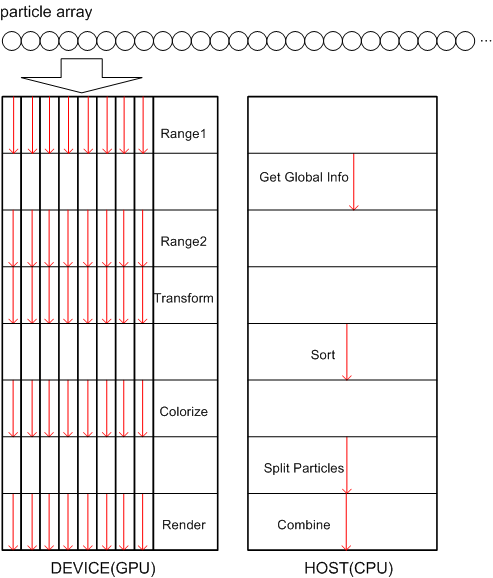
\includegraphics[width=0.50\textwidth]{cu_splotch_process.png}
\end{center}
\caption{Process of CUDA Splotch.}
\end{figure}

The overall process is illustrated in Figure 2. The red arrows show the 
execution of the processing steps. On the device side there are 
many arrows going together as CUDA threads running in parallel. In the
 Range step particle data are normalized and some global information is calculated, 
 like the maximum and minimum value of certain attributes. We let CPU handle
  the calculation of this as well as particle sorting after transformation.

After geometry transformation the area, or the location of the sub-image that each 
particle will influence is determined, and the empty sub-images will later be filled 
in the render step. Depending on the smoothing length of the particles and the 
camera settings the sizes of the sub-images range from 1*1 to the size of the 
final image, say 1000*1000, so the granularity of computing tasks in render step 
could be quite unbalanced. We found this unbalancing compromises speed, as shown in Table 3.

To solve that problem we imposed a new step on host, showing as 'Split Particles' 
in figure 2, to divide big tasks into smaller, average ones. Any particle
carrying a sub-image whose pixel number is larger than a barrier value will be 
splitted into multiple ones, each carrying a part of the pixels. The barrier value 
can be configured outside. In practical we found a number around the width 
or height of the final image, say 1024 usually works well.

There are of course cost for doing the splitting. The number of particles is 
increased which demands more thread issuing. Running the splitting algorithm itself
as well as the memory copying between host and device will also cost some time. 
Besides all these costs test results show that splitting brings speed increasing, as show in Table 3.

The output of rendering for the particles is stored in a one-dimension fragment buffer. 
After filled at the device-render step, fragment buffer is copied to host
 and combined to the final image by CPU. Here we found that the asynchronism of 
 device calling can be used to let device and host work in parallel. Say, when
rendering particle chunk N, combine the result of chunk N-1, the algorithm is listed below.

\begin{verbatim}
while  ( not all particles rendered )
{
       find the i-th subset S(i) in particle array that just uses up 
       fragment buffer;
A:     call device to render S(i);
       if  ( S(i) is not the first subset starting from index 0 )
       { 
B:          combine F(i-1), the output of S(i-1) in fragment buffer;
       }
C:     copy fragment buffer from device to host;
       if  ( S(i) is the last subset ending with index N, last index of
             particle array)
       {
             combine F(i);
       }
       i++;
}
\end{verbatim}


Instruction A is actually executed on device, which runs in parallel with 
instruction B, and the two paths merge at instruction C where they all have finished
. From test result we found that the combine time is mostly hidden by the render time.

In the future there are ways that worth trying to optimize CUDA Splotch. There are suggested, standard approaches
that can be tried to optimize CUDA Splotch, like unrolling short loops to optimize the control flow, using 
local/shared memory to accelerate data fetching and so on. As a parallel approach load-balancing is always an issue
which needs taking care of. For a system running CUDA, the load balance between CPU and GPU, and that between GPUs
should all be considered in order to obtain the full power of the hardware.



\section{Benchmarks}

The parallel Splotch code has been tested on different architectures and datasets, in order to 
exploit the various parallel approaches and to emphasize different characteristics of the software.

Taking advantage of the high portability of the code, we could perform our tests on a 5000 cores UNIX-AIX 
SP6 system, a cluster of 168 Power6 575 compute nodes with 32 cores per node and a memory of 128GB/node
(we will refer to this platform as SP6) and a Windows XP Machine with a CPU of Intel Xeon X5482 3.2 GHz and
2 GPUs of NVIDIA Quadro FX 5600 (indicated as Win). 
In this way, we can test the usage of Splotch on computing systems 
of different sizes and different target applications, from a standard PC (Win), where small-medium
data files can be used, up to 
a High Performance Computing platform where the huge and complex datasets can be processed.

Five different dataset have been used for the benchmarks. The first four are derived from 
the final output of a cosmological N-Body simulation, run using 870 millions of particles 
(fluid elements), characterized by their 3D coordinates and velocities, their mass density 
and the smoothing length, which defines the size of the region influenced by the properties
of each particle (see equation \ref{SPH:kern}). Subsets of 1, 10, 100 millions particles have been
randomly extracted from the whole dataset, producing three files of increasing size, indicated as
block1M, block10M and block100M. A fourth file, block870M contains the entire data product. 
Such variety of data sizes is necessary to match the memory requirements of the different available 
computing systems used used for the tests.

A further test has been performed using the final output of the MillenniumII simulation. 
This is our final reference benchmark, which consists in the visualization of a 10 billion
particle dataset.

All the data files are pure binaries, organized so that different quantitites are stored one after
the other in the file (e.g. $x$ coordinates of all particles are stored first, followed by $y$ 
coordinates and so on). In this way, we can easily adopt our MPI-IO based
reader. Only in the case of the MillenniumII data, we test also the native 
Gadget2 \cite{gadget} file format, using a integrated parallel version of the Gadget2 reader.

A summmary of the benchmarks is presented in table XXX. 

\begin{table}
\caption{Features of the datasets used in the benchmarks}
\begin{tabular}{|l|l|l|}
\hline
Label & 	N. particles & 	File size (Bytes)  \\
\hline
1M   & 	1000000   & 24000000 \\
\hline
10M  & 	10000000  & 240000000 \\
\hline
100M & 	100000000 & 2400000000 \\
\hline
850M & 	882739509 & 21185748216 \\
\hline
M-II & 	10000000000 & 	443456159744 \\
\hline
\end{tabular}
\end{table}


\subsection{MPI Benchmarks}

Table XX shows the test results on SP6 for dataset block 100M and block 870M.
Power6 cores can schedule two processes or threads in the same clock cycle, 
and it is possible to use a single core as two virtual CPUs. This mode of Power6 
is called Simultaneous Multi Threading (SMT).  This mode notably improves performance 
of process and rendering phases, reducing the execution time by 30%, but in I/O operations 
this reduction is lower and decreases as the chuncks of data to read grows.

Comparing MPI I/O reader with standard block reader, we see that improvements due to MPI2 functions 
appears when processes read large chunks of data. So good performances are expected as size of data increases.
Moreover when number of processes is high MPI I/O reader seems to perform and scale better than the other one.
   

\subsection{CUDA Benchmarks}

\begin{table}
\caption{Result of CUDA Splotch for benchmark 1M and 10M.}
\begin{tabular}{|l|l|l|l|l|}
\hline
	& setup/read(s) & 	drawing(s) & 	write(s) & 	total(s) \\
\hline
block 1M without CUDA & 	1.1259 & 	0.6982 & 	0.1860 & 	2.0103 \\
\hline
block 1M with CUDA & 	1.0916 & 	0.8411 & 	0.1840 & 	2.1170 \\
\hline
block 10M without CUDA & 	10.7064 & 	6.1376 & 	0.1842 & 	17.0284 \\
\hline
blocm 10M with CUDA & 	10.1411 & 	4.8261 & 	0.1865 & 	15.1537 \\
\hline
\end{tabular}
\end{table}

Table 2 shows the test result on Win for dataset block 1M and block 10M. For the
smaller dataset block 1M we can see that the speed with CUDA is slower than that without
it, because for small tasks the cost for applying CUDA can not be ignored, 
such as initialize CUDA runtime, data copying between host and device and so on. For block
10M we can see using CUDA gained us 21.3\% of speedup, here we define speedup as

speedup = (TimeWithoutCUDA - TimeWithCUDA)/TimeWithoutCUDA

CUDA(GPU) Splotch usually works better when handling the datasets
that generate visually appealing images like Figure 3, where drawing especially rendering
is a major work load. Table 3 shows some test result of such datasets. 
From the result we can see that CUDA provides a speedup to Splotch, and 
particle dividing helped improving the performance.


\begin{table}
\caption{Result of CUDA Splotch for small, middle and big datasets. The number of particle for the 
datasets, small=370,852, middle=2,646,991, big=16,202,527}
\begin{center}
\begin{tabular}{ | l || l | l || l | l | p{2cm} |}
\hline  
   &	CPU	& CPU	& GPU	& GPU	& GPU (no split)\\
\hline
  data & drawing time(s) & total time(s) & drawing time(s) & total time(s) & drawing time(s) \\
% without splitting(s) \\
\hline  
  small &	12.6419	& 13.0144	& 7.3885	& 7.7668	& 12.4894 \\
\hline
  middle &	18.5443 &	19.7190 &	11.3855 &	12.7118 &	16.6905 \\
\hline
  big	& 31.8976 &	39.3234 &	19.7792 &	27.0321	& 24.6305\\
\hline
\end{tabular}
\end{center}
\end{table}

\begin{figure}
\begin{center}
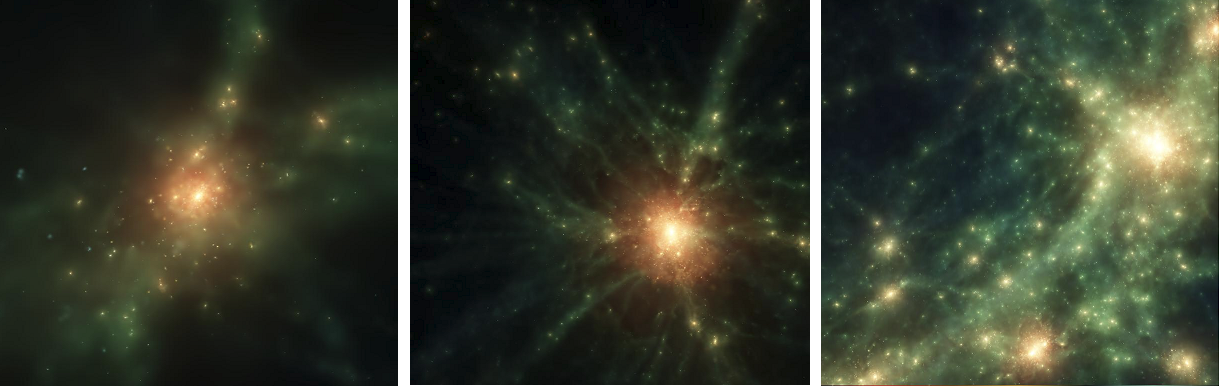
\includegraphics[width=1.0\textwidth]{cu_images.png}
\end{center}
\caption{Rendering result for small, middle and big datasets.}
\end{figure}


\begin{figure}
\begin{center}
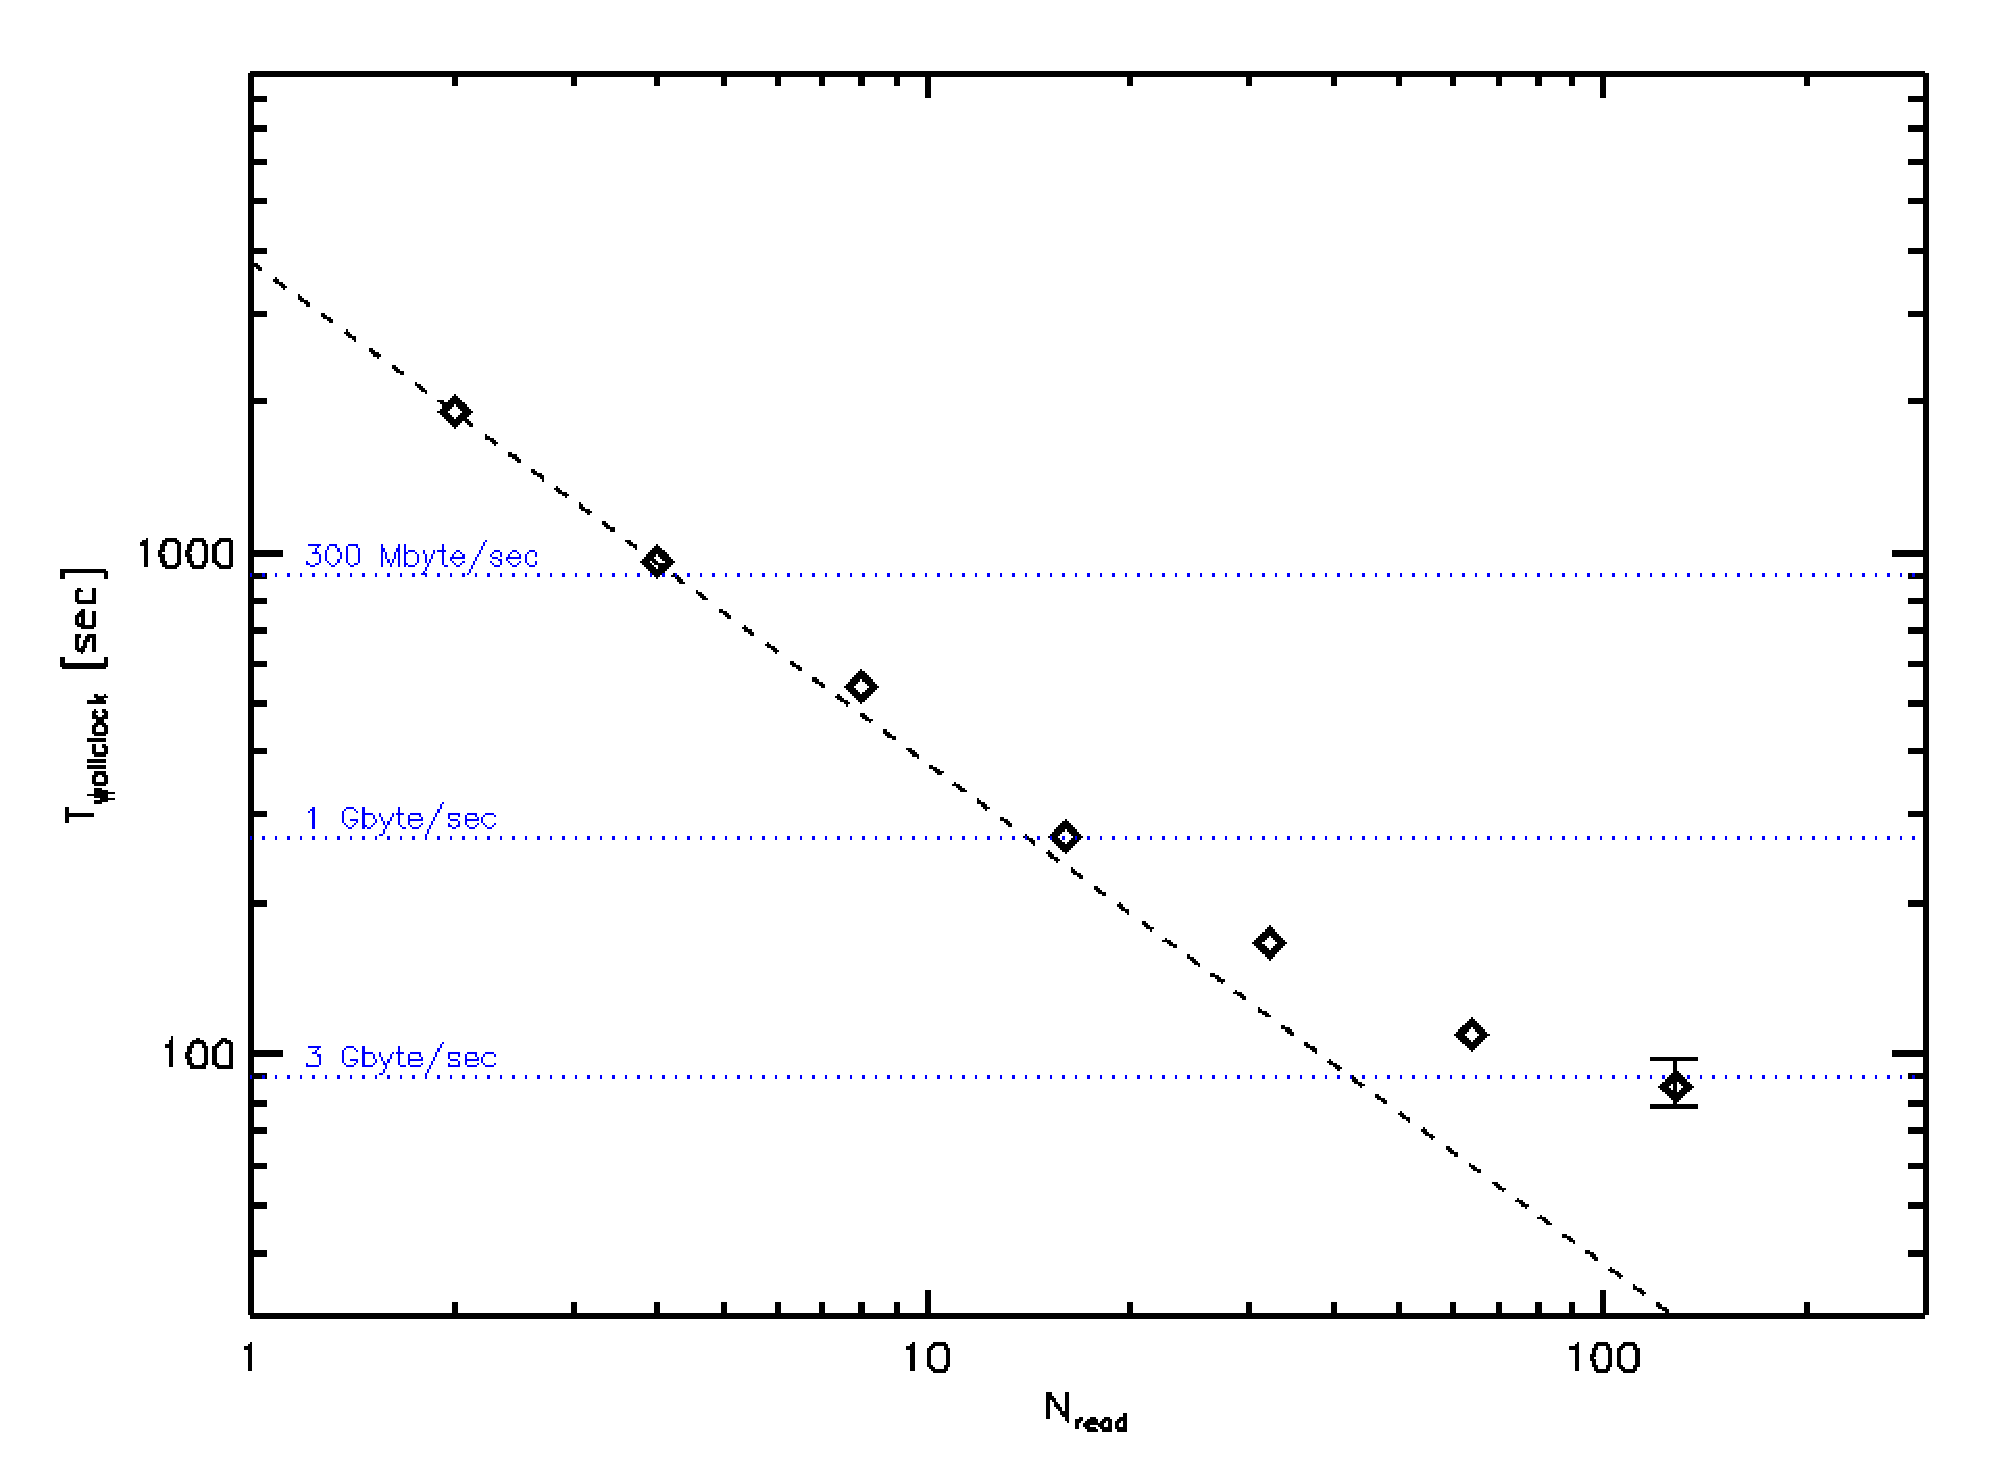
\includegraphics[width=0.5\textwidth]{t_cpu.pdf}
\end{center}
\caption{Shown is the scaling of the CPU time (total wallclock time substracting the time needed for 
readind and writing) with the number of MPI threads used for vizualisng 10 billion particles with an final
image size of 3200x3200 pixels. The dashed line indicates the expectation for an ideal scaling. The test was 
performed on a {\it Power6} architecture. The diamonds are runs using one task per core, the triangles indicate
using two tasks per core (a special feature of the {\it Power6} architecture), where we measure a speedup of 
a factor of 1.4.}\label{cpu_scaling}
\end{figure}

\begin{figure}
\begin{center}
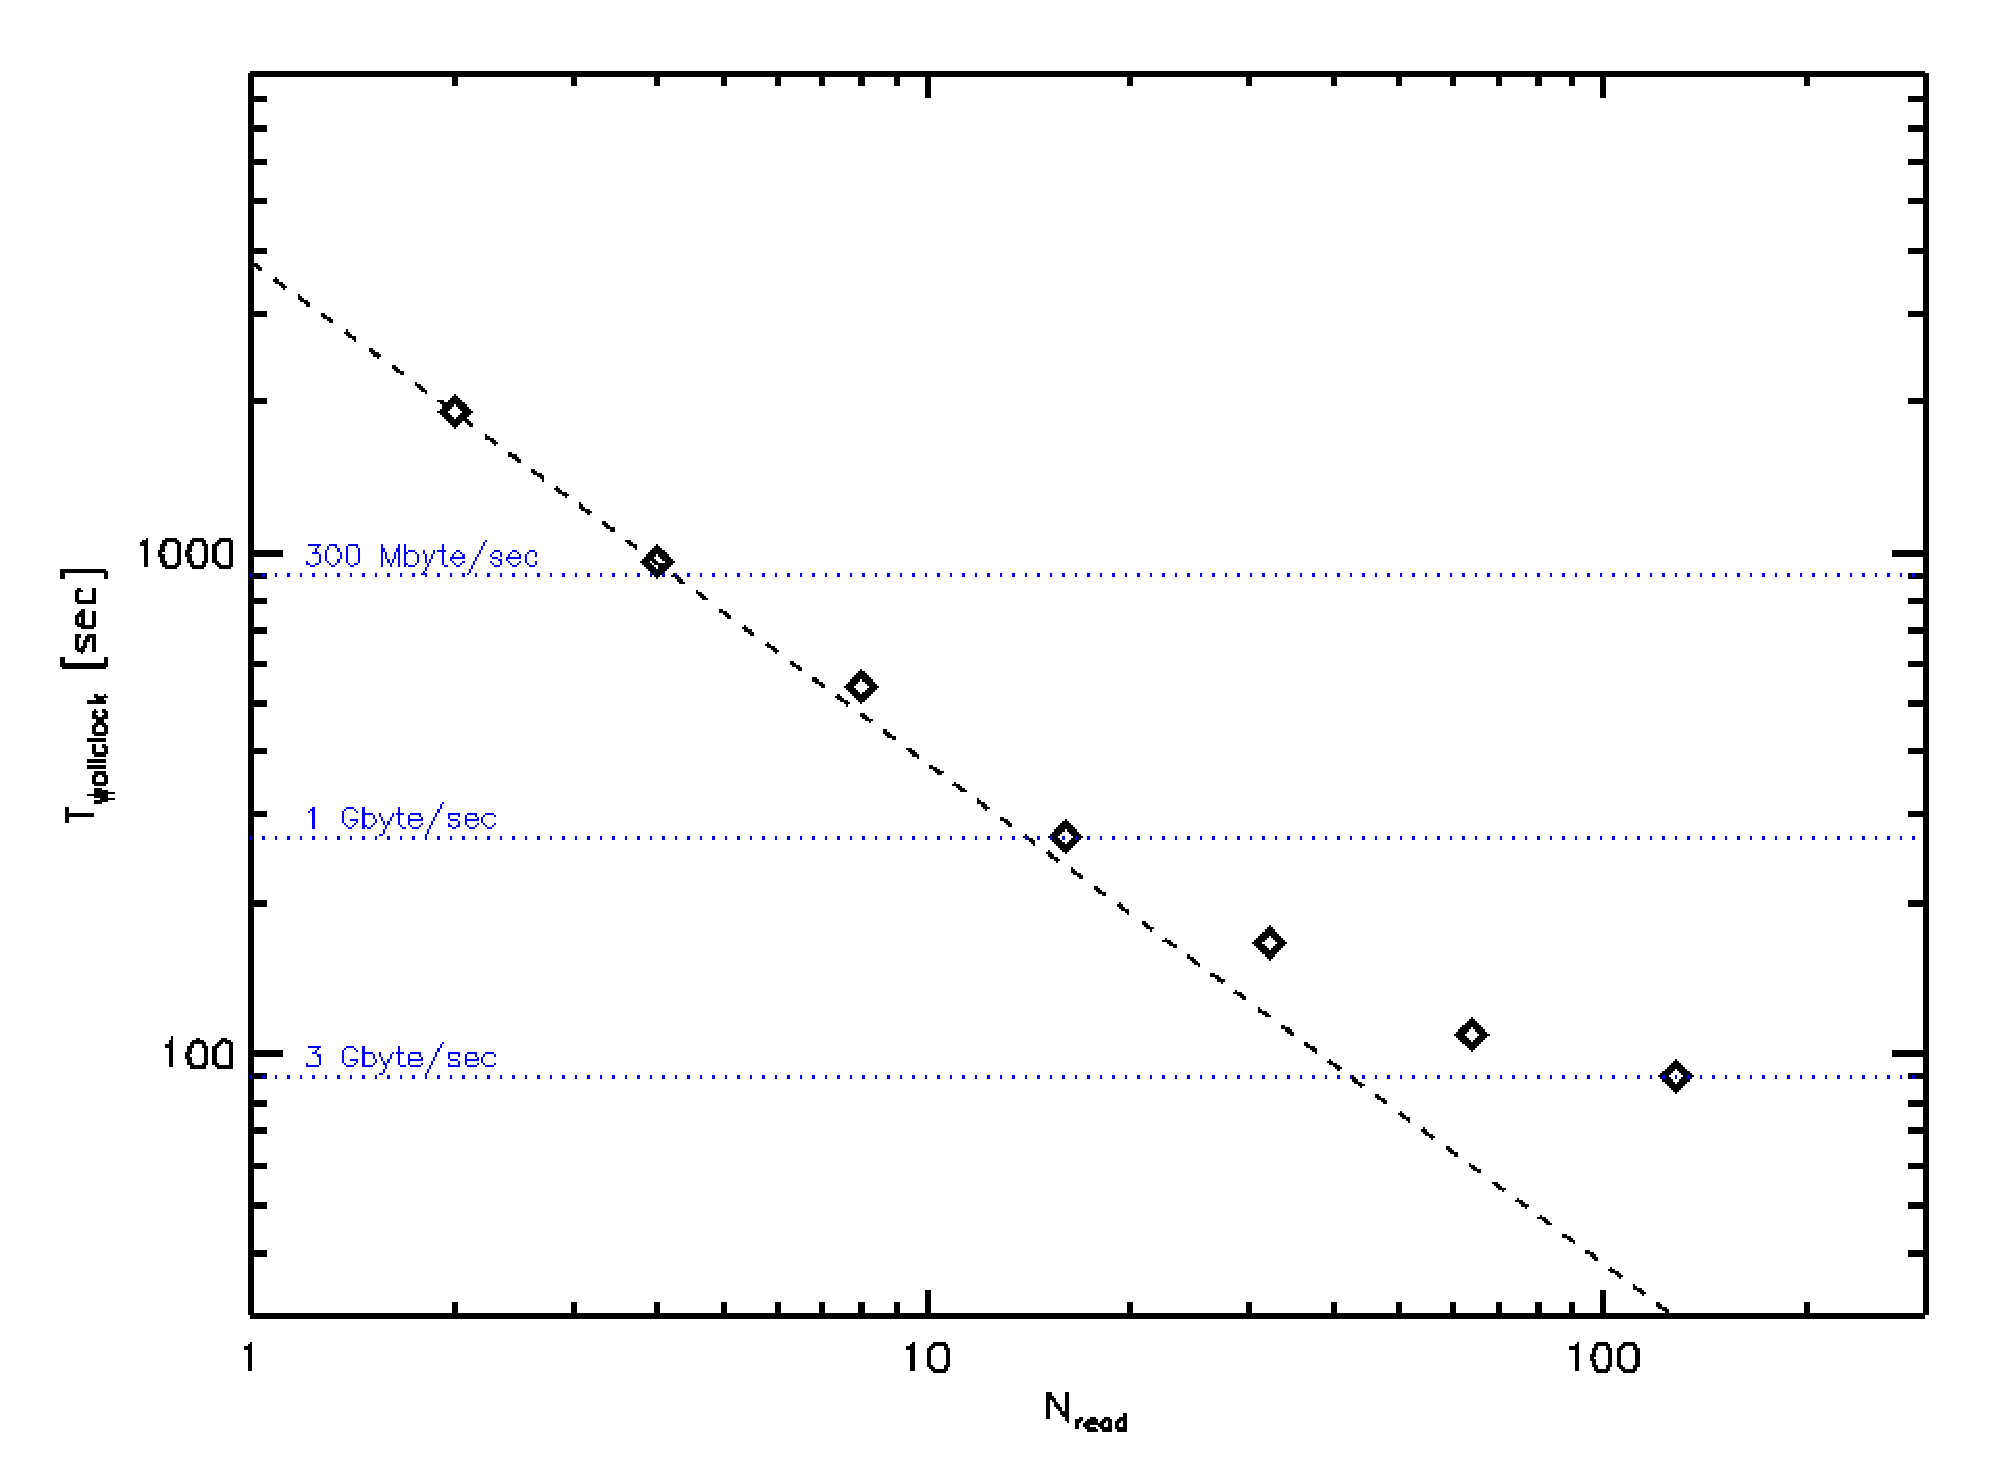
\includegraphics[width=0.5\textwidth]{t_read.pdf}
\end{center}
\caption{Shown is the scaling of the wallclock time needed to read the needed data 
(position, velocity and smoothing length) for the 10 billion particles of the simulation
as function of parallel reading tasks. The dashed line indicates the expectation for an 
ideal scaling. The horizontal lines indicate time expected for and IO throughput of 300 Mbype/sec,
1 Gbyte/sec and 3 Gbyte/sec. The read datapoint indicate the reading speed obtained if naively 
individual data elements are streamed instead of reading large blocks in juncks.}\label{read_scaling}
\end{figure}

\subsection{Visualization of the MillenniumII run}
\label{mII}



\section{Conclusions}
\label{conclusions}

Visualization is a powrful tool to explore in an immediate and 
effective way data, expecially large data, focusing on interesting or special features
which would be much harder to identify with a blind, systematic approach. 
Obviously, visualization cannot supersede quantitative analysis, however it helps in
understending the meaning and the content of complex digital information.

The continuously increasing data size and complexity requires more and more 
sophisticated visualization tools, able to appropriately render the information 
hidden in the files, which can process enormous data volumes, such those produced 
by ultimate scientific experiments or computer simulations.

Splotch matches both requirements. It produces high quality image output,
based on a ray tracing algorithm specifically designed to exploit at best the 
properties of point-like data distributions. Furthermore, it can run on a large 
variety of high performance computing architectures, thanks to its hybrid
parallel implementation, which can take advantage of multi-processors system, adopting
an MPI based approach, multi-core shared memory processors, exploiting OpenMP,
GPUs, relying on CUDA. This allows to achieve high performance overcoming the typical
memory barriers posed by small personal systems, commonly adopted for visualization.
Finally, Splotch is written in ANSI C++ and is compeltely self-contained (it does not
require any complementary library, apart from MPI, OpenMP and CUDA stuff). 
This make the code easily portable and compilable over a large number of different 
architectures and operating systems. The next steps will be that of porting and 
running Splotch on hybrid system, multiprocessor computers with GPUs, exploiting 
both MPI and CUDA on the same dataset.

We have tested Splotch on datasets of different sizes. In particular we manage to 
visualize the largest cosmological simulation currently available, the MillenniumII run, 
processing 10 billions particle in a single shot.

\section*{Acknowledgments}
We would like to thank Mike for providing the data of the MilleniumII simulations 
on which we conducted our perfgomance tests. K.~D.~acknowledges the
supported by the DFG Priority Programme 117. Finally, we acknowledge 
HPC Europa 2 project, funded by the European Commission - 
DG Research in the Seventh Framework Programme under grant agreement n� 228398, 
for the committed resources.

\section*{References}


%% References with BibTeX database:
\begin{thebibliography}{00}

%\bibliographystyle{elsarticle-num}
%\bibliography{master.bib}

%% Authors are advised to use a BibTeX database file for their reference list.
%% The provided style file elsarticle-num.bst formats references in the required Procedia style

%% For references without a BibTeX database:



\bibitem{sdss} http://www.sdss.org/

\bibitem{lofar} http://www.lofar.org/

\bibitem{2009MNRAS.398.1150B} Resolving cosmic structure formation with the Millennium-II Simulation,
Boylan-Kolchin M., Springel V., White S.~D.~M., Jenkins A., Lemson G., 2009, Monthly Notices of the Royal Astronomical Society, 398, 1150-1164

\bibitem{lsst}http://www.lsst.org/lsst

\bibitem{iraf} http://iraf.noao.edu/

\bibitem{midas} http://www.eso.org/sci/data-processing/software/esomidas/

\bibitem{sao} http://tdc-www.harvard.edu/software/saoimage.html

\bibitem{gaia} http://astro.dur.ac.uk/~pdraper/gaia/gaia.htx/index.html

\bibitem{gnuplot} http://www.gnuplot.info/

\bibitem{supermongo} http://www.astro.princeton.edu/~rhl/sm/sm.html

\bibitem{idl} http://www.ittvis.com/

\bibitem{survey} XXX

\bibitem{paraview} http://www.paraview.org/

\bibitem{aladin} http://aladin.u-strasbg.fr/

\bibitem{topcat} M. B. Taylor, TOPCAT \& STIL: Starlink Table/VOTable Processing Software, ASP, ASPC 347 29T, 2005

\bibitem{visivo1}Visualization, Exploration and Data Analysis of Complex Astrophysical Data,
M. Comparato, U. Becciani, A. Costa, B. Garilli, C. Gheller, B. Larsson, J. Taylor, 2007, 
The Publications of the Astronomical Society of the Pacific, Volume 119, Issue 858, pp. 898-913.

\bibitem{3dslicer} M. A. Borkin, N. A. Ridge, A. A. Goodman and M. Halle, Demonstration of the Applicability of 3D Slicer to Astronomical Data using 13CO and C18O Observations of IC348, astro-ph/0506604, 2005

\bibitem{splash} http://users.monash.edu.au/~dprice/splash/index.html

\bibitem{visit} https://wci.llnl.gov/codes/visit/

\bibitem{visivo2}VisIVO-Integrated Tools and Services for Large-Scale Astrophysical Visualization, U. Becciani, A. Costa, V. Antonnuccio-Delogu, G. Caniglia, M. Comparato, C, Gheller, Z. Jin, M. Krokos, P. Massimino, The Publications of the Astronomical Society of the Pacific, (to appear).

\bibitem{simbad} http://simbad.u-strasbg.fr/simbad/

\bibitem{vizier} http://cdsarc.u-strasbg.fr/viz-bin/VizieR

\bibitem{2008NJPh...10l5006D}Splotch: Visualizing Cosmological Simulations. K.Dolag, 
M. Reinecke, C.Gheller, S. Imboden, 2008, New Journal of Physics, Volume 10, Issue 12, pp. 125006

\bibitem{mpi} http://www.mpi-forum.org/

\bibitem{openmp} http://openmp.org/

\bibitem{cuda} http://www.nvidia.com/object/cuda\_home.html

\bibitem{rvn} http://ibm-deep-computing-visualization-rvn-end.software.informer.com/

\bibitem{gadget} Springel V 2005 Monthly Notices of the Royal Astronomical Society 364, 1105-1134

\bibitem{1985A&A...149..135M} A refined particle method for astrophysical problems, 
Monaghan J.~J. \& Lattanzio J.~C., 1985, A\&A, 149, 135

\bibitem{1991par..book.....S} Physics of Astrophysics: Volume I Radiation, Shu F., 1991,
Published by University Science Books, 648 Broadway, Suite 902, New York, NY 10012


\end{thebibliography}

\end{document}

%%
%% End of file `procs-template.tex'.
